% \section{\rnn Development Context}\label{sec:context}
\chapter{\textcolor{red}{The ATLAS Detector}}\label{sec:context}



The ATLAS experiment~\cite{PERF-2007-01}\footnote{\textcolor{red}{ATLAS uses a right-handed coordinate system with its origin at the nominal interaction point (IP) in the centre of the detector and the z-axis along the beam-pipe. The x-axis points from the IP to the centre of the LHC ring, and the y-axis points upward. Cylindrical coordinates (r, $\phi$) are used in the transverse plane, \phi being the azimuthal angle around the beam-pipe. The pseudorapidity is defined in terms of the polar angle $\theta$ as \eta = -$\ln{tan(\theta/2)}$. The angular distance $\Delta R$ is defined as $\Delta R = \sqrt{(\Delta\eta)^{2} + (\Delta\phi)^{2}}$ . Transverse momenta and energies are defined as $pT = p\sin\theta$ and $E_{T}$ = $E\sin\theta$, respectively}.} is designed to observe particles
produced in high-energy proton--proton collisions and, hereby not addressed,
heavy-ion LHC collisions. Its calorimeter system comprises both 
electromagnetic (ECAL) and hadronic (HCAL)
sections (Section~\ref{ssec:calo}), which overlap an inner detector. The two-level triggering system reduces the total
data-taking rate \textcolor{red}{from 40 MHz} to approximately \textcolor{red}{1 kHz. Here}, we focus on electron-based channels, which are
found in many interesting physics phenomena, \textcolor{red}{such as the} the decays of the Higgs
boson~\cite{HIGG-2012-27,HIGG-2016-33}, for instance.
% A trigger system sequential 
%logic dedicated to
%select collision events containing physics objects with specific
%properties is  referred to select collision events containing physics objects
%with specific properties are referred to as trigger, and the complete
%configuration of the triggers, operating in parallel, is called the trigger
%menu, with a specific set for each trigger level.



The standard variables for electron identification are discussed in
Section~\ref{ssec:std_variables}. The electron triggers are described in
Section~\ref{ssec:egamma_trigger}, followed by their nomenclature in
Section~\ref{ssec:menu}.  Considerations about the \TnP method
(Section~\ref{ssec:tnp}) and datasets (Section~\ref{ssec:dataset}) employed \textcolor{red}{to extract signal and background samples
from real ATLAS data} close this section.




\section{Calorimeter System}\label{ssec:calo}


%
\begin{table}[p]\scriptsize
\centering
\caption{\label{tab:granularity}Acceptance region, granularity, longitudinal
  segmentation and number of readout cells in the ATLAS calorimetry system. The
  total number of readout cells is 187,652 (178,308) with (without) the
  pre-sampler calorimeter. Provided number of readout cell account for both
end-cap sides. Adapted from~\cite{PERF-2014-07}.}%
\resizebox{.90\textwidth}{!}{%
  \begin{tabular}{m{4cm} m{2cm} m{2.5cm} m{2.5cm}}
  \hline
  \hline
  \hline
  \textbf{Pre-sampler (\ps)} & \textbf{Barrel}        &      \textbf{End-cap} & \\
 EM section & (\presamplerb) & (\presamplere) \\
  \hline
  \hline
  Acceptance   &  $\abseta<1.52$ & $1.5<\abseta<1.8$   \\
  \hline
  Longitudinal Segmentation & 1 sampling  & 1 sampling  \\
  \hline
  Granularity ($\Delta \eta \times \Delta \phi$)    &  $0.025 \times \pi/32$ &
  $0.025 \times \pi/32$  \\
  \hline
  Number of readout cells & 7,808 & \multicolumn{2}{l}{1,536} \\
  \hline
  \hline
  \textbf{LAr Accordion}  (\ecal) & \textbf{Barrel} &
  \textbf{End-cap}  \\
  EM section  &   (\emb)         &       (\emec) \\
  \hline
  \hline
  & \multicolumn{2}{c}{Total Acceptance} & Partial Acceptance \\
  \cline{2-4}
            &  $\abseta<1.475$ & $1.375<\abseta<3.2$   \\
  \hline
  & \multicolumn{2}{c}{Longitudinal Acceptance} \\
  \cline{2-4}
  & \multicolumn{1}{l|}{\multirow{3}{2cm}{3 samplings}}  & 3 samplings & $1.5   < \abseta < 2.5$ \\
  \cline{3-4}
  & \multicolumn{1}{l|}{} & 2 samplings & $1.375   < \abseta < 1.5$ \\
  \cline{3-4}
  & \multicolumn{1}{l|}{} & 2 samplings & $2.5     < \abseta < 3.2$ \\
  \hline
  \multicolumn{4}{c}{Granularity ($\Delta \eta \times \Delta \phi$)}  \\
  \hline
  \multirow{6}{4cm}{$1^{\underline{\text{st}}}$ longitudinal sampling (\emi)}  &
   \multicolumn{1}{l|}{$0.025/8 \times \pi/32 $}  & $0.050 \times \pi/32$ & \hspace{-0.1cm}$1.375 < \abseta < 1.425$ \\
  \cline{3-4}
            & \multicolumn{1}{l|}{}  & $0.025 \times \pi/32$ & $1.425   < \abseta < 1.5$ \\
  \cline{3-4}
  & \multicolumn{1}{l|}{$ \abseta<1.4 $}  & $0.025/8 \times \pi/32$ & $1.5   < \abseta < 1.8$ \\
  \cline{2-4}
            & \multicolumn{1}{l|}{$0.025 \times \pi/128 $} & $0.025/6 \times
            \pi/32$ & $1.8   < \abseta < 2.0$ \\
  \cline{3-4}
  & \multicolumn{1}{l|}{} & $0.025/4 \times \pi/32$ & $2.0   < \abseta < 2.37$ \\
  \cline{3-4}
            & \multicolumn{1}{l|}{$ 1.4<\abseta<1.475 $} & $0.1 \times
            \pi/32$ & $2.37  < \abseta < 3.2$ \\
   \cline{1-4}
   \multirow{4}{5cm}{$2^{\underline{\text{nd}}}$ longitudinal sampling (\emii)}  &
							\multicolumn{1}{l|}{$0.025 \times \pi/128$}& $0.050 \times \pi/128$ & \hspace{-0.1cm}$1.35 < \abseta < 1.425$ \\
	\cline{3-4} &
  \multicolumn{1}{l|}{$\abseta<1.4$} & $0.025 \times \pi/128$   & $1.425 < \abseta < 2.5$ \\
	\cline{2-4}
            &   \multicolumn{1}{l|}{$0.075 \times \pi/128$}              &
            \multirow{2}{2.5cm}{$0.1 \times \pi/32$} & \multirow{2}{2.5cm}{$2.5 < \abseta < 3.2$} \\
            &   \multicolumn{1}{l|}{$1.4 < \abseta < 1.475$}       & \\
  \cline{1-4}
  \multirow{2}{*}{$3^{\underline{\text{rd}}}$ longitudinal sampling (\emiii)} &
  \multicolumn{1}{l|}{$0.050 \times \pi/128$} &
  \multirow{2}{*}{$0.050 \times \pi/128$}
  & \multirow{2}{*}{$1.5   < \abseta < 2.5$} \\
  & \multicolumn{1}{l|}{$\abseta < 1.35$} & & \\
  \hline
  Number of readout cells & 101,760 & \multicolumn{2}{l}{62,208} \\
   \hline
   \hline
   \textbf{Scintillating Tiles} (\tilecal)  & & \textbf{Barrel}  & \textbf{Extended
   Barrel}     \\
   HAD section & & (\tilebar) & (\tileext) \\
   \hline
   \hline
  Total Acceptance &  &  $\abseta<1.0$ & $0.8<\abseta<1.7$   \\
   \hline
  Longitudinal Segmentation & & 3 samplings  & 3 samplings  \\
   \hline
  \multicolumn{4}{c}{Granularity ($\Delta \eta \times \Delta \phi$)}  \\
  \hline
  \multicolumn{2}{l}{$1^{\underline{\text{st}}}$ (\hadi) and
  $2^{\underline{\text{nd}}}$ (\hadii) longitudinal samplings}
  &  $0.1 \times \pi/32$ & $0.1 \times \pi/32$   \\
  \cline{1-4}
  $3^{\underline{\text{rd}}}$ longitudinal sampling (\hadiii) & &  $0.2 \times \pi/32$ &
  $0.2 \times \pi/32$   \\
  \hline
  Number of readout cells & & 2,880 & \multicolumn{1}{l}{2,304} \\
  \hline
  \hline
  \textbf{Intermediate \tilecal} (\itc) &  Crack Region & & \\
  \hline
  \hline
  Total Acceptance & \multicolumn{3}{l}{${\sim}0.8 < \abseta < 1.6$} \\
  \hline
  Special Segmentation & \multicolumn{3}{l}{Contains 24 readout cells in a $\eta$
  slice. Within them, the
  scintillating stabs.} \\
  \hline
  \hline
  \textbf{LAr Plates}   &  &  \textbf{End-cap}     \\
  HAD section														&  & (\hec) 				 \\
  \hline
  \hline
  Total Acceptance  &   & $1.5<\abseta<3.2$  \\
  \hline
  Longitudinal Segmentation &   & 4 samplings  \\
  \hline
  \multicolumn{4}{c}{Granularity ($\Delta \eta \times \Delta \phi$)}  \\
	 & & & Partial Acceptance \\
  \hline
  \multirow{2}{*}{All longitudinal samplings} & \multicolumn{1}{l|}{} & $0.1 \times \pi/32 $ & $1.5 < \abseta < 2.5$ \\
  \cline{3-4}
  & \multicolumn{1}{l|}{} & $ 0.2 \times \pi/16 $ & $ 2.5 < \abseta < 3.2$ \\
  \hline
  Number of readout cells & & \multicolumn{2}{l}{3,564} \\
  \hline
  \hline
  \textbf{Forward Calorimeters}  &  &
  \multicolumn{2}{l}{\textbf{Forward Region}}    \\
  \hline
  \hline
  Total Acceptance &  & $ 3.1 < \abseta < 4.9 $ \\
  \hline
  Longitudinal Segmentation &   & 3 samplings \\
  \hline
  Granularity ($\Delta \eta \times \Delta \phi$)& &
  \multicolumn{2}{l}{${\sim}0.2\times\pi/16$} (varies on $\eta$) \\
  \hline
  Number of readout cells & & \multicolumn{2}{l}{1,762} \\
  \hline
  \hline
  \hline
\end{tabular}
}
\end{table}






The calorimeter system covers the pseudorapidity
range \(|\eta| < 4.9\)~\cite{PERF-2007-01}. Within the region \(|\eta|< 3.2\),
electromagnetic calorimetry is provided by barrel and endcap high-granularity
lead/Liquid-Argon (LAr) calorimeters, with an additional thin LAr presampler
(\ps) covering \(|\eta| < 1.8\), in order to correct for energy losses in
material upstream of the calorimeters~\cite{LARG-2009-01,larg_tdr}. Hadronic
calorimetry is provided by \textcolor{red}{a} the steel/scintillating-tile calorimeter
(\tilecal~\cite{TCAL-2017-01,tile_tdr}), \textcolor{red}{constituted} of three barrel structures
within \(|\eta| < 1.7\), and two copper/LAr hadronic endcap calorimeters
(\hec)~\cite{cal_tdr}.  The solid angle coverage is completed with forward
copper/LAr and tungsten/LAr calorimeter modules optimised for electromagnetic
(EM) and hadronic (HAD) measurements, respectively. The specified calorimeters
provide full azimuthal ($\phi$) coverage with a total of about 190,000 \textcolor{red}{readout cells. Transition regions between calorimeters are used to locate detector services and induce a sharing of showers between calorimeters that degrades energy measurements in those regions. In particular,} the transition from the barrel to the end-cap within
$1.37<|\eta|<1.52$ is complemented by scintillator stab ($1.0<|\eta|<1.6$) to
estimate signal losses~\cite{cal_tdr}.

The electromagnetic and hadronic systems comprise three sampling layers each along longitudinal (depth) segmentation ~\cite{PERF-2007-01}\footnote{The two
central layers in HCAL end-cap are summed to result in a single measurement.}.
Each sampling layer has its own lateral ($\eta\times\phi$) granularity (see Table~\ref{tab:granularity}, for detailed information). Besides granularity, the amount of material in front of the detector in each sampling layer also vary with \abseta, leading to variable expected lateral and longitudinal profiles. \textcolor{red}{Additionally}, the expected
profile is also dependent on the physics object total energy. \textcolor{red}{In the EM calorimeter}, most of \textcolor{red}{the EM shower} energy is collected in the second layer, while the third layer provides measurements
of energy deposited in the shower tails. %as shown in Figures~\ref{fig:cal_em_x0} and~\ref{fig:cal_had_lambda}.

%, which
%may vary with $\eta$. This is particularly true for the first EM layer, which
%provides fine-grained granularity on $\eta$, since its strip cells would become
%physically too narrow to keep the same granularity starting from $|\eta|>1.8$
%(from 8 cells to 6 in a region of $\Delta\eta=0.025$), and further losing
%granularity after $\abseta>2.0$ (4 cells). The strips are only available for
%$\abseta<2.37$ and offer excellent discrimination between photons and
%$\pi^{0}\to\gamma\gamma$ decays. 

%Besides granularity, the amount of material in
%front of the detector and in each sampling layer may also vary with \abseta, as
%shown in Figures~\ref{fig:cal_em_x0} and~\ref{fig:cal_had_lambda}, leading to
%variable lateral and longitudinal profiles. 
%Particularly, the expected profile is also
%dependent on the physics object total energy. 
%At lowest unprescaled electron
%triggers~\cite{ATL-DAQ-PUB-2018-002}, most of energy is collected in the second
%layer, while the third layer provides measurements of energy deposited in the
%shower tails. 
The hadronic calorimeters, which surround the EM detectors,
provide additional discrimination power through further energy measurements of
possible EM shower tails, as well as rejection of events with activity of
hadronic origin with three sampling layers. Although calorimeters are designed 
to have uniform response for full detector acceptance, there are residual fluctuations 
dependent on the shower development position~\cite{Wigmans2017}.


\begin{comment}
\begin{figure}[ht]
  \centering
  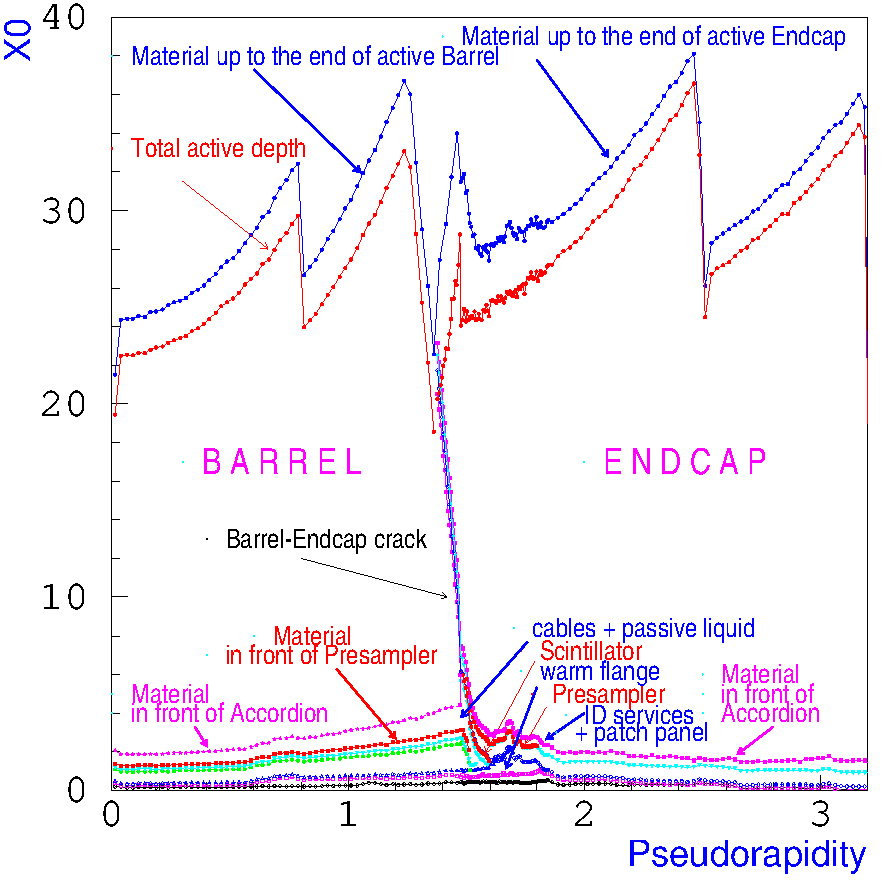
\includegraphics[width=.5\textwidth]{sections/context/figures/cal_em_x0.pdf}
  \caption{Simulation of accumulated radiation lengths ($\text{X}_0$), as a function of \abseta for several detectors or materials.The material is given in
terms of $\text{X}_0$ and $\lambda_{\text{int}}$ to decrease material-dependent
effects in the reported dimensions of the calorimeter
absorbers.%Simulation of accumulated radiation lengths ($\text{X}_0$), as a function of
  %\abseta for several detectors or materials. $\text{X}_0$ is defined as the
  %distance over electrons (or positrons) loses ${\sim}\SI{63.2}{\%}$ (average)
  %of their energy~\cite{Wigmans2017}. 
  Extracted from~\cite{cal_tdr}.}%
  \label{fig:cal_em_x0}
  \end{figure}
  
  \begin{figure}[ht]
  \centering
  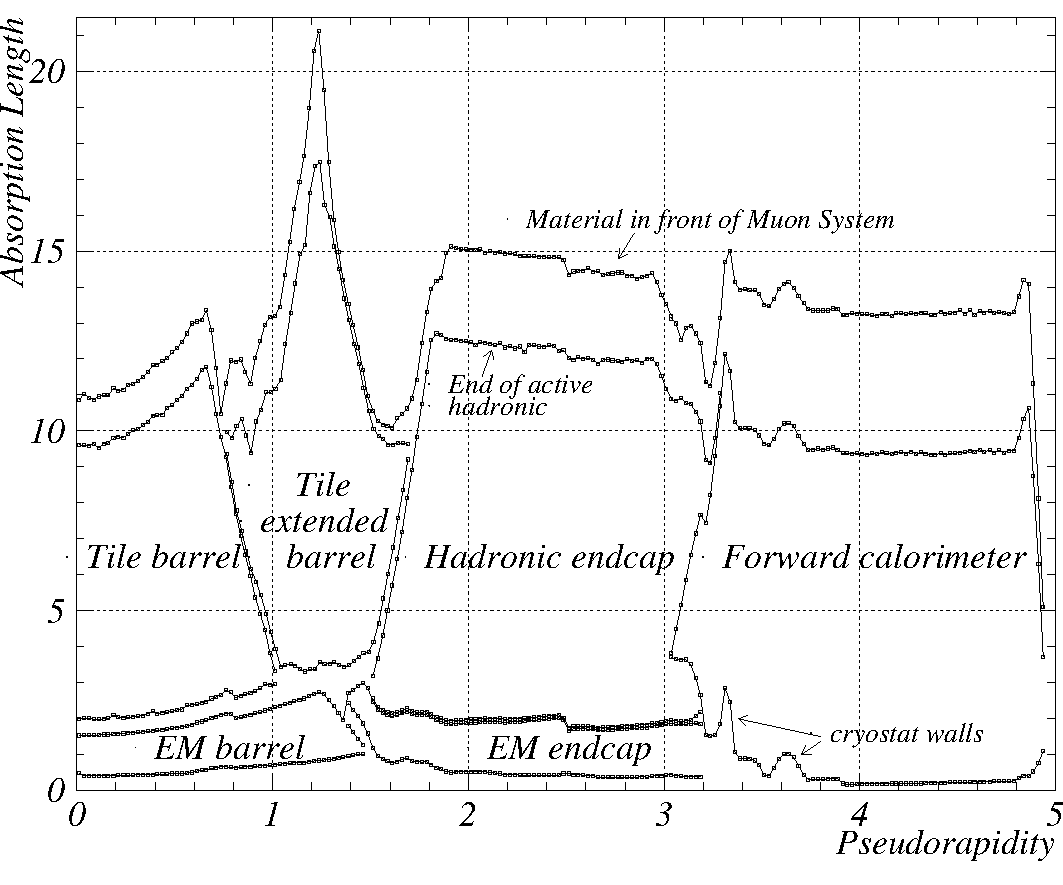
\includegraphics[width=.5\textwidth]{sections/context/figures/cal_had_lambda.pdf}
  \caption{Simulation of accumulated nuclear interaction length ($\lambda_{int}$),
    as a function of \abseta{} for several detectors or materials.
  $\lambda_{\text{int}}$ is defined as the average distance a hadron has to
  travel within the medium before a nuclear interaction
  occurs~\cite{Wigmans2017}. Extracted from~\cite{cal_tdr}.}%
  \label{fig:cal_had_lambda}
\end{figure}
\end{comment}


\subsection{Inner Detector}\label{ssec:track}

The inner detector, \textcolor{red}{used to reconstruct charged-particle tracks}, is immersed in a
\textcolor{red}{\SI{2}{\tesla} magnetic} field \textcolor{red}{aligned on the beam axis and produced} by a thin superconducting solenoid
and covers a pseudorapidity range $|\eta| \lesssim 2.5$~\cite{PERF-2007-01}.
Three technologies are employed, with thinner granularity nearer to the
interaction point~\cite{PERF-2015-08,inner_tdr1,inner_tdr2}: \textcolor{red}{a} Pixel Detector (92
million channels), \textcolor{red}{a} Silicon Microstrip Detector (SCT, 6.3 million channels) and
\textcolor{red}{a} Transition Radiation Detector (TRT, 350 thousand channels). The TRT offers
electron identification capability within its pseudorapidity coverage ($|\eta|
\lesssim 2$) via the detection of transition-radiation photons \textcolor{red}{generated at the interface between the radiator material and detection straws.} Track reconstruction requires (pile-up \textcolor{red}{and the event topology} dependence) CPU intensive
computations due to the complexity of image-processing algorithms \textcolor{red}{fighting against combinatorial backgrounds when associating hits to tracks ~\cite{PERF-2015-08}. In} 2016, it was the second
most-demanding reconstruction algorithm in the \hlt{}.






\section{Standard Electron Identification Variables}\label{ssec:std_variables}

The specificities of the signal and background interaction processes with
detector instrumentation can be used to construct meaningful and discrimination
efficient physics variables. Except for the hardware-based calorimeter trigger
and the \rnn (Section~\ref{sec:neuralringer}), electron
identification~\cite{atlas_electron_id_offline} relies on the variables
described in Table~\ref{tab:IDcuts}. 
%A schematic illustration of the ATLAS components employed on these variables can be seen in Figure~\ref{fig:schematic_id_inputs}. 
The cut-based algorithm in electron
triggers applies thresholds on the three most discriminating discussed in Table~\ref{tab:IDcuts}. They describe the shape of the electromagnetic shower: \reta{}, \eratio{}, \rhadone{}.



\begin{table*}
%\caption{Definitions of electron discriminating variables, the types of backgrounds the variables help to discriminate against, and if a variable is used as a likelihood pdf ($\mathcal{L}$) or used as a rectangular cut (C). The $^{*}$ refers to the fact that the $E/p$ and \wstot variables are
%  only used for electrons with $\pt > 150~\GeV$ for the \Tight identification operating point (in software release 20.7), and are not used for the looser operating points.}
\caption{Type and description of the quantities used in electron
  identification.  The columns labelled ``Rejects'' indicate whether a quantity
  is used to discriminate prompt electrons from light-flavour (LF) jets, photon
  conversions ($\gamma$), or non-prompt electrons from the semileptonic decay of
  hadrons containing heavy-flavour (HF) quarks ($b$- or $c$-quarks).  In the
  column labelled ``Usage,'' an ``LH'' indicates that the probability density
  estimation (pdf) of this quantity
  is used in forming $\mathcal{L}_{s}$ and $\mathcal{L}_{b}$ (defined in
  Eq.~(\ref{eq:likelihoods})) and a ``C'' indicates that this quantity is used
  directly as a selection criterion.  In the description of the quantities
  formed using the second layer of the calorimeter, 3$\times$3, 3$\times$5,
  3$\times$7, and 7$\times$7 refer to areas of $\Delta\eta \times \Delta\phi$
  space in units of $0.025 \times 0.025$. Extracted from~\cite{aaboud2019electron}
}%
\label{tab:IDcuts}
\scriptsize
%\renewcommand{\arraystretch}{1.}
\begin{center}
\resizebox{\textwidth}{!}{%
\begin{tabular}{|l|l|l|c|c|c|l|}
\hline
Type & Description & Name &  \multicolumn{3}{c|}{Rejects} & Usage  \\
 & & & LF & $\gamma$ & HF &\\
\hline
 Hadronic & Ratio of \et in the first layer of the hadronic calorimeter  & \rhadone & x & & x & LH \\ 
 leakage & to \et of the EM cluster & & & & & \\
& (used over the range $|\eta| < 0.8$ or $|\eta| > 1.37$)  & & & & & \\
\cline{2-7}
  & Ratio of \et in the hadronic calorimeter &  & & & & \\
  &  to \et of the EM cluster & \rhad & x & & x & LH  \\
 & (used over the range $0.8 <|\eta| < 1.37$) & & & & & \\
\hline
Third layer of  & Ratio of the energy in the third layer to the total energy in the & & & & &\\
EM calorimeter  & EM calorimeter. This variable is only used for & & & & & \\
& $\et < \SI{80}{\GeV}$, due to inefficiencies at high \et, and is& \fIII & x & & & LH \\
                & also removed from the LH for $|\eta| > 2.37$, where it is& & & & & \\
                & poorly modelled by the simulation. & & & & & \\
\hline
Second layer of  & Lateral shower width, $\sqrt{(\Sigma E_i \eta_i^2)/(\Sigma E_i) -((\Sigma E_i\eta_i)/(\Sigma E_i))^2}$, & & & & & \\
EM calorimeter  & where $E_i$ is the energy and $\eta_i$ is the pseudorapidity  & \weta & x & x & & LH \\
 & of cell $i$ and the sum is calculated within a window of 3$\times$5 cells & & & & & \\
\cline{2-7}
& Ratio of the energy in 3$\times$3 cells over the energy in 3$\times$7 cells & \rphi & x & x & x & LH  \\
& centred at the electron cluster position & & & & & \\
\cline{2-7}
& Ratio of the energy in 3$\times$7 cells over the energy in 7$\times$7 cells  & \reta & x & x & x & LH  \\
& centred at the electron cluster position & & & & & \\
\hline
First layer of       & Shower width, $\sqrt{(\Sigma E_i (i-i_\mathrm{max})^2)/(\Sigma E_i)}$, where $i$ runs over  &   & & & & \\  
EM calorimeter       & all strips in a window of $\Delta\eta \times \Delta\phi \approx 0.0625 \times 0.2$,   & \wstot & x & x & x & C \\
		     & corresponding typically to 20 strips in $\eta$, and $i_\mathrm{max}$ is the & & & & &                  \\
		     & index of the highest-energy strip, used for \et\ $>$ 150~\gev\ only        &  & & & &   \\
\cline{2-7}
                     & Ratio of the energy difference between the maximum &    & & & &  \\
                     & energy deposit and the energy deposit in a secondary & \deltaEmax & x & x & & LH  \\
                     & maximum in the cluster to the sum of these energies & & & & &   \\
\cline{2-7}     
& Ratio of the energy in the first layer to the total energy  & \fI & x & & & LH  \\
& in the EM calorimeter &  & & & & \\
\hline
Track  & Number of hits in the innermost pixel layer &   $n_\mathrm{Blayer}$ & & x & & C \\
%conditions & &   $ $  & & & & \\
%discriminates against photon conversions &   $ $  & & & & \\
\cline{2-7}
conditions                     & Number of hits in the pixel detector        &    $n_\mathrm{Pixel}$ & & x & & C \\
\cline{2-7}
                     & Total number of hits in the pixel and SCT detectors  &   $n_{\mathrm{Si}}$  & & x & & C \\
\cline{2-7}
                     & Transverse impact parameter relative to the beam-line
		     % cut-based: trackd0_physics:Transverse impact parameter with respect to the beam spot,
		     % LH: el_trackd0pvunbiased and el_tracksigd0pvunbiased
		                                                  &       \trackdO  & & x & x & LH \\
\cline{2-7}
                     & Significance of transverse impact parameter &       |\dOSignificance|  & & x & x & LH  \\
                     & defined as the ratio of \trackdO to its uncertainty                     &  & & & &              \\
\cline{2-7}
                     &  Momentum lost by the track between the perigee and the last &   \deltapoverp & x & & & LH \\
                     & measurement point divided by the  momentum at perigee & & & & & \\
\hline
%TRT                 & Total number of hits in the TRT      & $n_\mathrm{TRT}$          \\
%\cline{2-3}
%TRT                 & Ratio of the number of high-threshold hits to the total number of  hits in the TRT &    \TRTHighTHitsRatio  \\
%\cline{2-3}
TRT                       & Likelihood probability based on transition radiation in the TRT &   \TRTPID & x & & & LH  \\
\hline
Track--cluster     & $\Delta\eta$ between the cluster position in the first layer &   \deltaeta & x & x & & LH  \\
matching          &  and the extrapolated track & & & & &   \\
%\cline{2-3}
%  matching    & $\Delta\phi$ between the cluster position in the middle layer and the extrapolated & \deltaphires\\
%&   track, where the track momentum is rescaled to the cluster energy &  \\
%&   before extrapolating the track to the middle layer of the calorimeter  &  \\
%\cline{2-7}
%     & $\Delta\phi$ between the cluster position in the middle layer and & \deltaphi & x & x & & $\mathcal{LH}$  \\
%  & $ $and the track extrapolated from the perigee & & & & & \\
%\cline{2-7}
%&   Defined as  \deltaphi, but the track momentum is rescaled &   & & & &  \\
%&   to the cluster energy before extrapolating the track from  & \deltaphires & x & x & & $\mathcal{LH}$  \\
%&   the perigee to the middle layer of the calorimeter  & & & & &  \\
\cline{2-7}
&   $\Delta\phi$ between the cluster position in the second layer &   & & & &  \\
&   of the EM calorimeter and the momentum-rescaled  & \deltaphires & x & x & & LH  \\
&   track, extrapolated from the perigee, times the charge $q$  & & & & &  \\
\cline{2-7}
                    & Ratio of the cluster energy to the track momentum, used for            &       $E/p$   & x & x & & C\\
                    & \et $>$ 150~\gev\ only & & & & &  \\
%\hline
%Conversions         & Veto electron candidates matched to reconstructed photon  conversions            &  isConv \\
\hline
\end{tabular}
}
\end{center}
\end{table*}




\begin{comment}

\begin{figure}[t]
  \begin{center}
  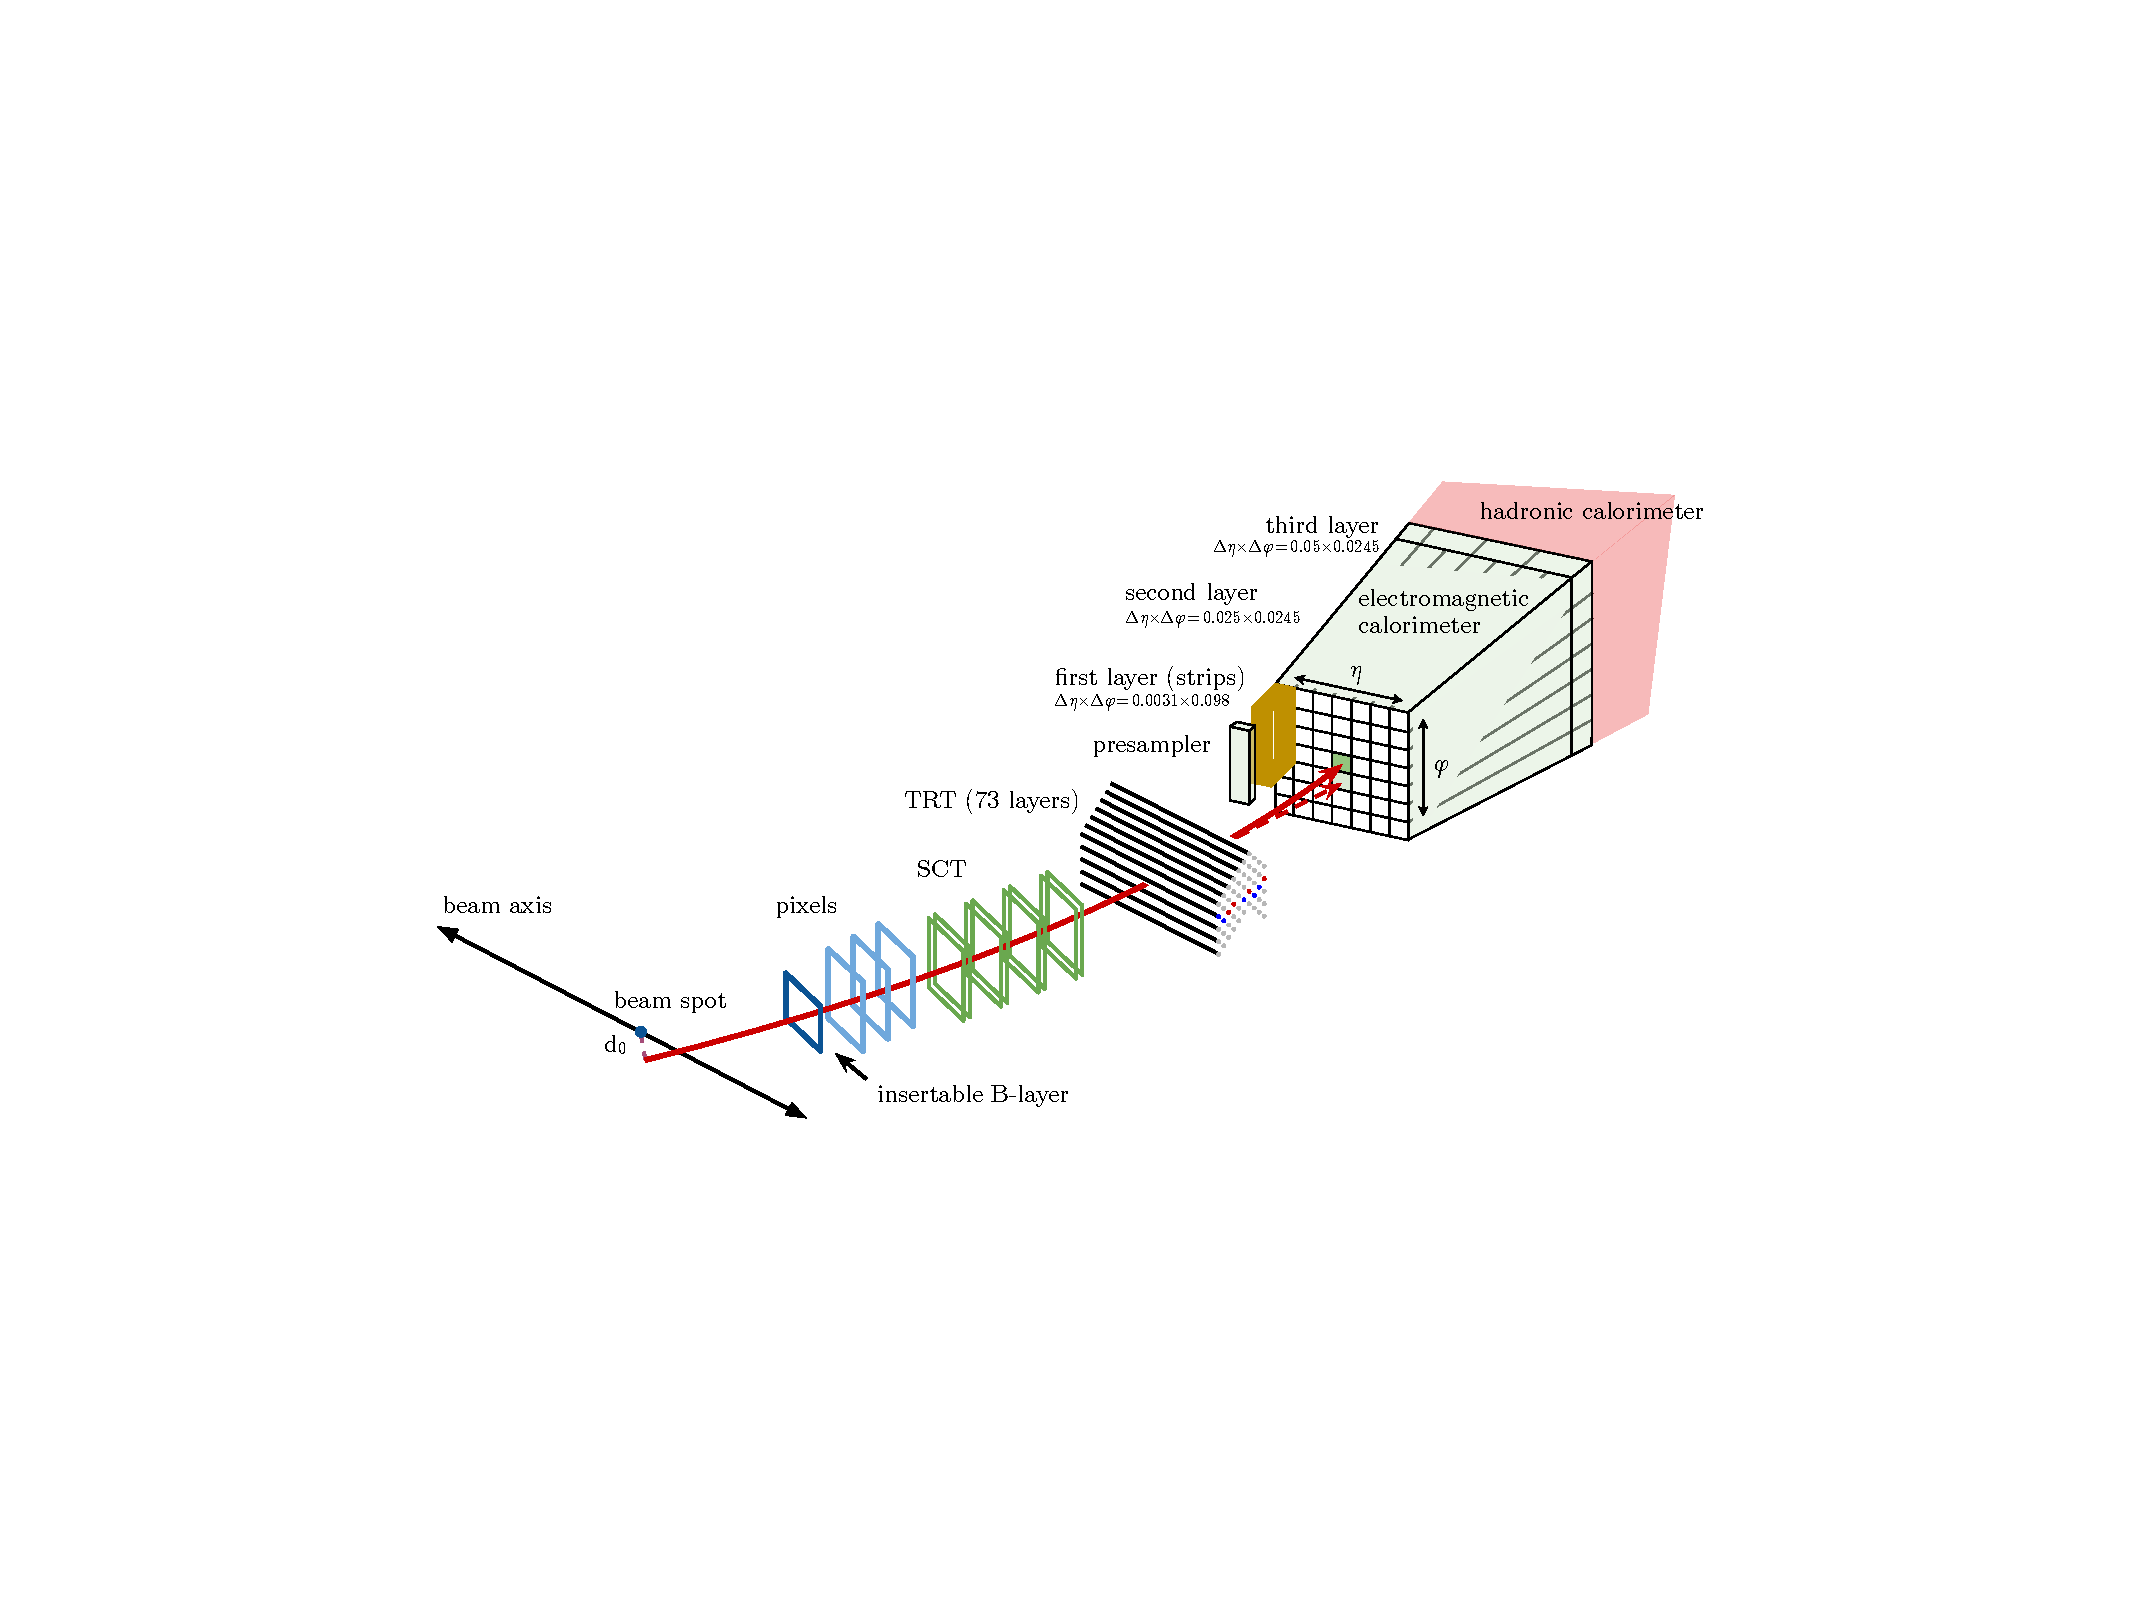
\includegraphics[width=0.98\textwidth]{sections/context/figures/electron_variables_3rdLayerGranularity_v2_noPhantom_noVars}
  %electron_variables_3rdLayerGranularity_v2_noPhantom}
  %%%\includegraphics[width=0.98\textwidth]{figaux_03}
  \caption{
  A schematic illustration of the path of an electron through the detector.
  The red trajectory shows the hypothetical path of an electron, which first traverses
  the tracking system (pixel detectors, then silicon-strip detectors and lastly the TRT)
  and then enters the electromagnetic calorimeter.
  The dashed red trajectory indicates the path of a photon produced by the interaction of
  the electron with the material in the tracking system.
  Extracted from~\cite{aaboud2019electron}.
  %This figure also describes various inputs used to form the electron-identification quantities, such as \reta\, \rphi, and \TRTPID, as will be described in Table~\ref{tab:IDcuts} of Section~\ref{sec:identification}.
  }%
  \label{fig:schematic_id_inputs}
  \end{center}
\end{figure}
\end{comment}  




  
The standard electron identification variables are based on in-depth
understanding of the signatures left by signal and background.  As a result, information in specific regions of the experiment
\textcolor{red}{are fused together using a set of a few variables (i.e. 3
variables for describing the shower shape in the EM2). The objective is to reduce the dimensionality of the problem} and compose a highly discriminant input space to apply a set of rectangular cuts, which provides a simple yet powerful selection mechanism. The use of variables providing similar information
(i.e. correlated) is discouraged, once they usually do not aggregate with
discriminating power and make analysis more
complex~\cite{aaboud2019electron}.

In the end of the \textcolor{red}{LHC} Run~1~\cite{PERF-2016-01}, the strategy for offline electron identification was improved by the adoption of a multivariate approach, which computes a likelihood discriminant. Here, an approximation is made by \textcolor{red}{assuming} the statistical independence between variables ~\cite{kendalls_vol2b}. This likelihood approach was also brought to the final HLT selection in Run 2 (Section~\ref{ssec:egamma_trigger}) to improve overall efficiency. that approximates inference through the
%hypothesis of statistical independence between variables~\cite{kendalls_vol2b}.
%The likelihood computation~\cite{aaboud2019electron} allows to account for
%the presence of both background-like and signal-like variables, but also to
%benefit from additional discriminant power of similar variables. It was extended
%to the final HLT selection in Run 2 (Section~\ref{ssec:egamma_trigger}) to
%improve overall efficiency. In other words, the strategy for improving the
%selection of electrons was either obtained by finding better ways of defining
%the decision boundary upon available variables (i.e. use of a multivariate
%approach) or by searching for a new variable to complement or replace previous
%ones. Nevertheless, the approach for defining discriminant variables remained
%the same.




In a broader sense, other ATLAS physics objects (i.e. taus and jets) \textcolor{red}{have successfully}, for
which discrimination relies on less prominent instrumentation and carried out on
similar signal--background interactions, have successfully applied other
multivariate methods (i.e. boosted decision-trees and neural-networks) for
modelling a more suitable (and complex) decision boundary
%~\cite{Radovic2018,ATLASCollaboration2017f,ATLASCollaboration2018c,
%ATLASCollaboration2017g,ATLASCollaboration2016,tau_run2_rnn_bdt}.

\section{Feature Extraction: Ring Sums}\label{ssec:concept}

%One disadvantage of this strategy is that it requires discriminant information
%to be captured through variables that are individually conceived to explore
%specific physics or instrumentation knowledge. By alleviating this requirement,
%other variables can be conceived while still affording from field-specific
%knowledge.
%We take advantage of field-specifc knowledge to follow another path.
%\textcolor{red}{The create the rins sums it was} taken into account the approximately conical structure of the shower to
%construct energy quantities describing the total energy deposited in a
%concentric ring of cells (\figurename~\ref{fig:calo_rings}), or simply ring, 
At each calorimeter sampling layer, the energy deposition of an incoming particle is extracted by building concentric rings of cells (\figurename~\ref{fig:calo_rings}), or simply rings. All rings in the \ecal sampling layers are
\textcolor{red}{centered around their most} energetic (hottest) cell, a reasonable
approximation of the energy barycenter of the \textcolor{red}{shower for} online
\textcolor{red}{operation. Focusing on EM objects, rings are} built using as axis center the position of
the hottest cell in the second electromagnetic \textcolor{red}{layer, collecting the largest fraction} of the total absorbed electron energy.

The ring building process covers the whole $0.4\times0.4$ (\etaphi axis) RoI
seeded by \licalo, resulting in \textcolor{red}{100 rings. The number of rings}
naturally varies per calorimeter sampling layer, as shown in
\tablename~\ref{tab:ring_alg_parameters}, to account for different layer
granularity. Thereby, a dimensionality reduction is provided by compacting
typical input space dimensionality of approximately 1000--1200 cells per ROI into
the above-mentioned 100 rings through the usage of \textcolor{red}{EM shower} physics \textcolor{red}{knowledge: the rings} can keep a complete description of the (symmetric) lateral and
longitudinal information. However, the algorithm only approximates this concept
in order to meet the online operation requirements and avoid further
manipulation of the instrumented information. The full description and
discussion on the current algorithm are addressed in
Section~\ref{top:algorithm}.



\begin{table}[ht!]
\centering
\caption{Nomenclature defining the ringer algorithm layers and sections, as well
  as the respective parameters employed and calorimeter sampling
  layers from which the cells are extracted. The ringer algorithm
  parameters are dependent on the ringer layer $l$ and independent on \eta{} and
  \et{} during Run~2. The parameters are the ring size in \eta{}
  ($h_{\etaa,l}$), $\phi$ ($h_{\phii,l}$) and the number of rings to be computed
  in each layer ($\text{N}_l$). The values for $h_{\etaa,l}$ and $h_{\phii,l}$
  are approximated, the exact ones can be obtained for $\eta=0$ in
  Table~\ref{tab:granularity}.
%To refer to a ring, it will be used notation XYYY, where X is the ring index in
%the YYY layer.
}%
\label{tab:ring_alg_parameters}
\resizebox{.8\textwidth}{!}{%
\begin{tabular}{lc|ccc|ccc}
\hline
\hline
\multicolumn{2}{c|}{Ringer} & \multicolumn{3}{c|}{Calorimeter Sampling} & 
\multicolumn{3}{c}{Parameters} \\
\hline
Section & Layer ($l$) & Barrel & \itc & End-cap & $h_{\etaa,l}$ & $h_{\phii,l}$ & $N_l$ \\
\hline
\hline
\multirow{4}*{EM} & \ps &  \presamplerb & & \presamplere & 0.025 & 0.1 & 8 \\
\cline{2-5}
& \emi & \emb{1} &  & \emec{1} & 0.003 & 0.1 & 64  \\
\cline{3-5}
& \emii & \emb{2} &  & \emec{2} & 0.025 & 0.025 & 8 \\
\cline{3-5}
& \emiii & \emb{3} &  & \emec{3} & 0.050 & 0.025 & 8 \\
\cline{1-5}
\multirow{6}*{HAD} & \multirow{2}*{\hadi} & \tilebar{0} &
\multirow{2}*{\tilegap{3}} & \multirow{2}*{\hec{0}} & \multirow{2}*{0.1} & \multirow{2}*{0.1} & \multirow{2}*{4} \\
&                     & \tileext{0} &                               &                           \\
\cline{3-5}
& \multirow{2}*{\hadii} & \tilebar{1} & \multirow{2}*{\tilegap{1}} & \hec{1}       & \multirow{2}*{0.1} & \multirow{2}*{0.1} & \multirow{2}*{4} \\
&                   & \tileext{1} &              & \hec{2}  \\
\cline{3-5}
& \multirow{2}*{\hadiii} & \tilebar{2} & \multirow{2}*{\tilegap{2}} & \multirow{2}*{\hec{3}} & \multirow{2}*{0.2} & \multirow{2}*{0.1} & \multirow{2}*{4} \\
&                     & \tileext{2} &                &             \\
\hline
\hline
\end{tabular}
}
\end{table}





\begin{figure}[h!t]
	\centering
	\begin{center}
		\begin{subfigure}[c]{0.8\textwidth}
			\centering
			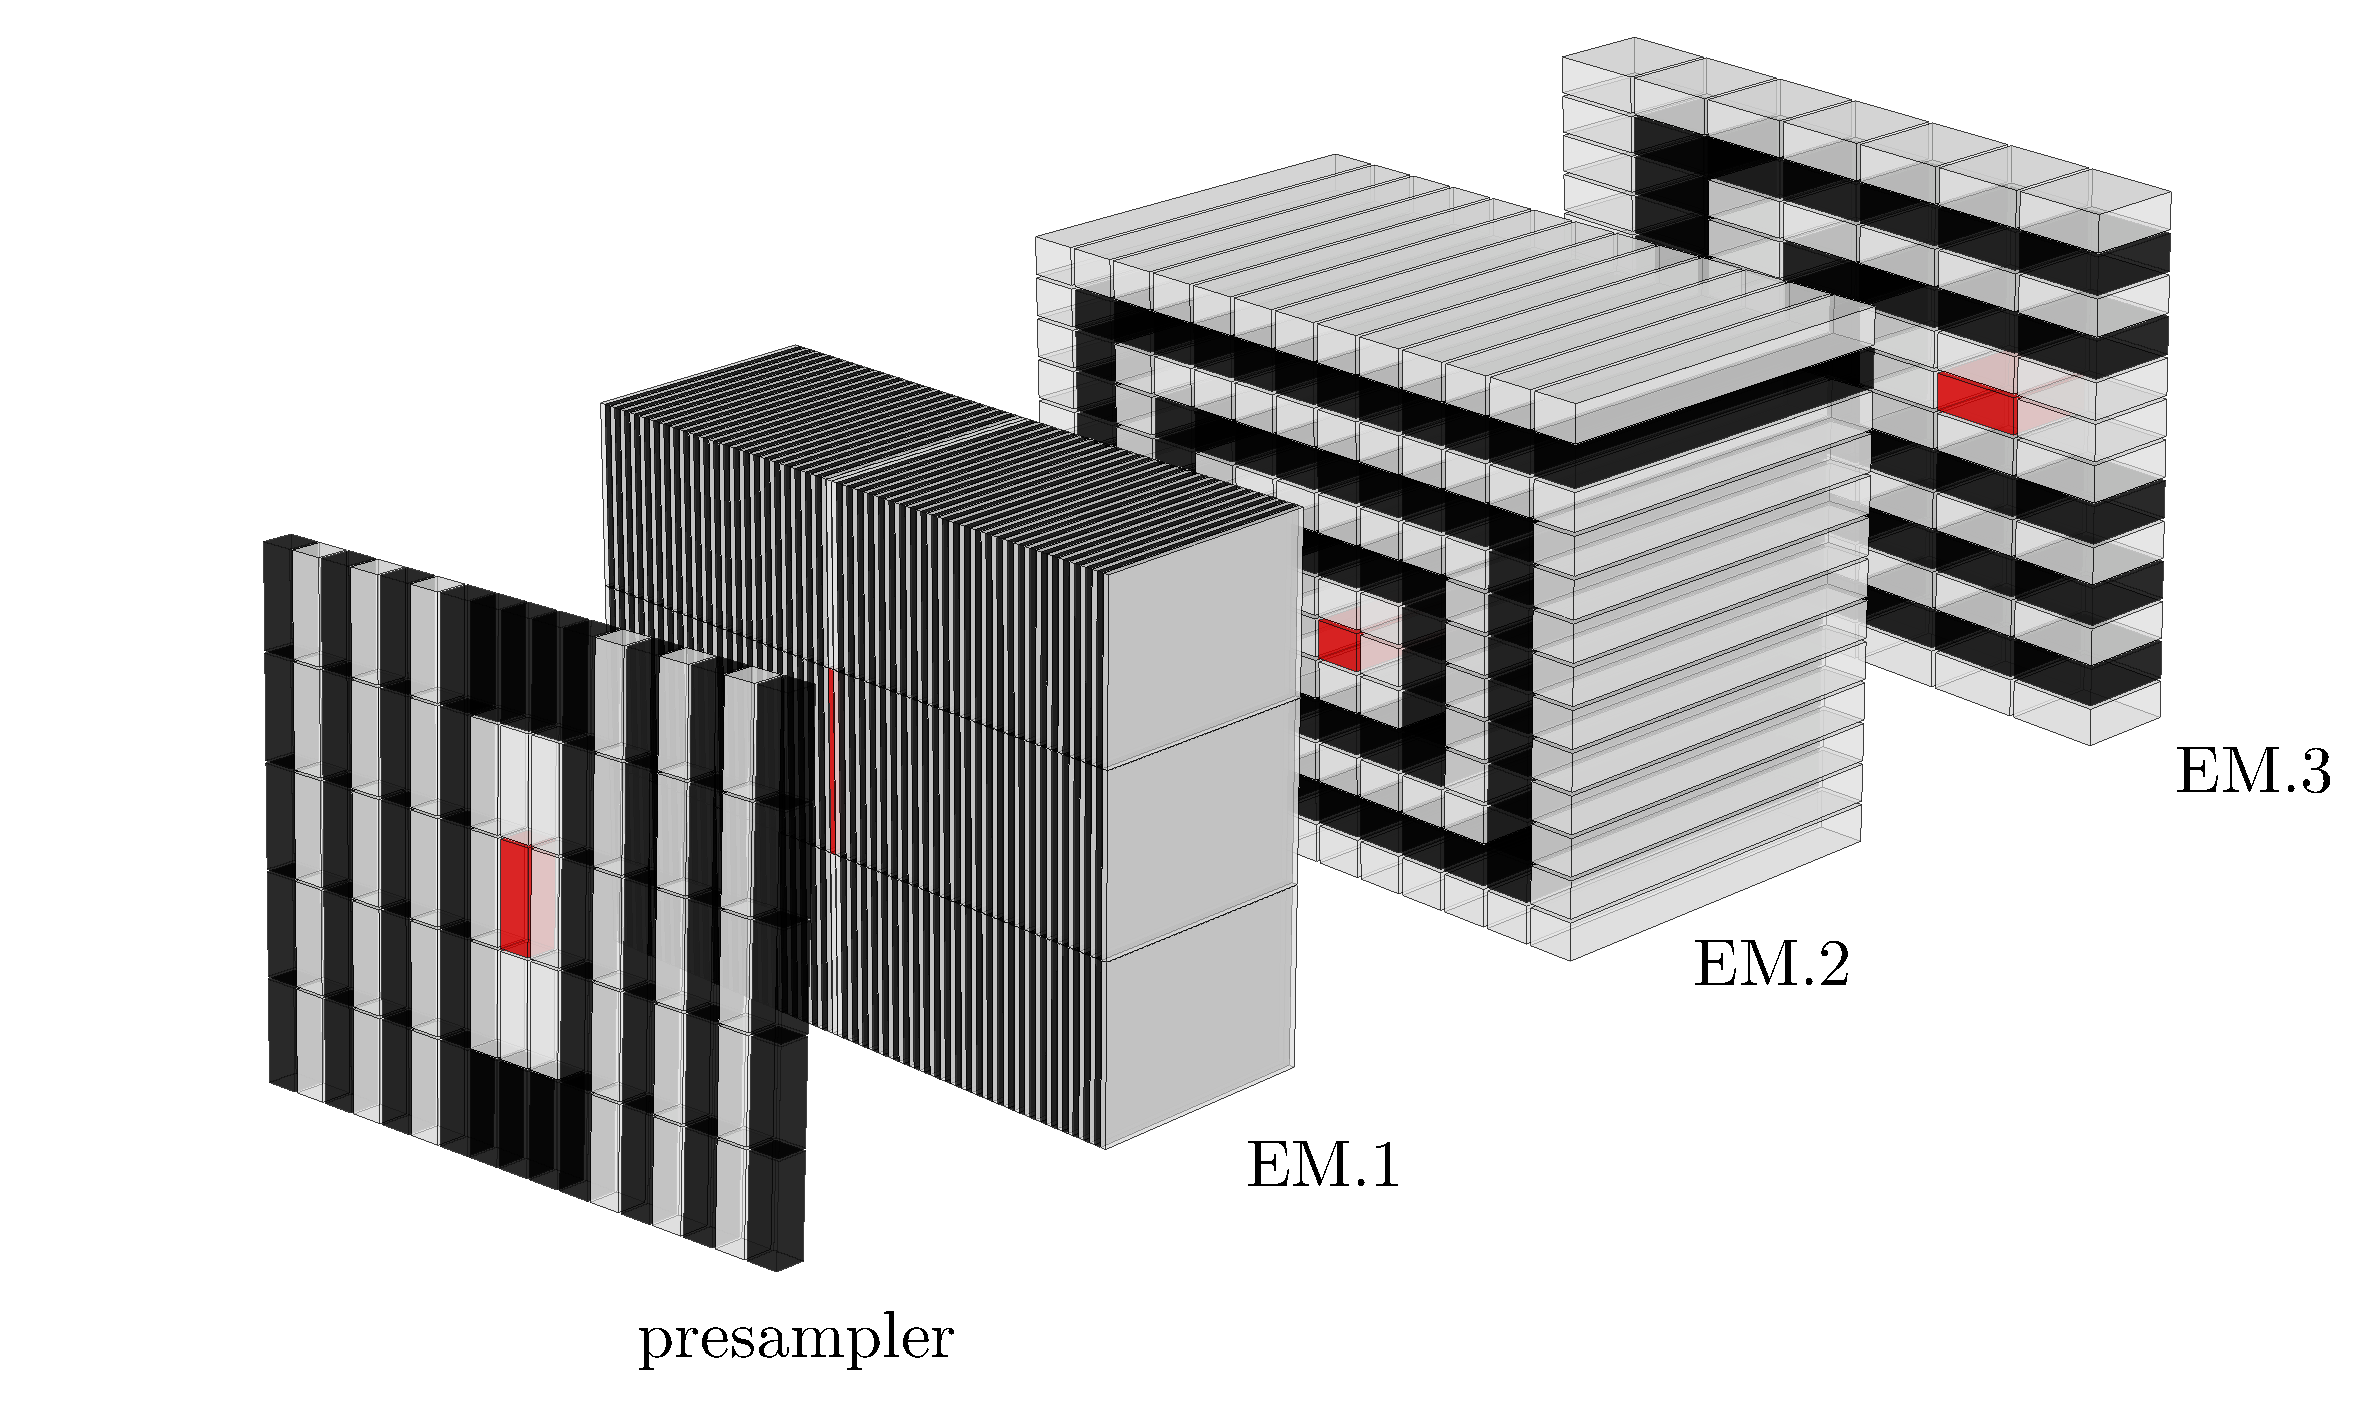
\includegraphics[width=\textwidth]{sections/ringer/figures/ATLAS_EM_Layers_v5.pdf}
			\caption{Eletromagnetic calorimeter cells within the ringer reconstruction window.}
		\end{subfigure} \\
		\begin{subfigure}[c]{0.8\textwidth}
			\centering
			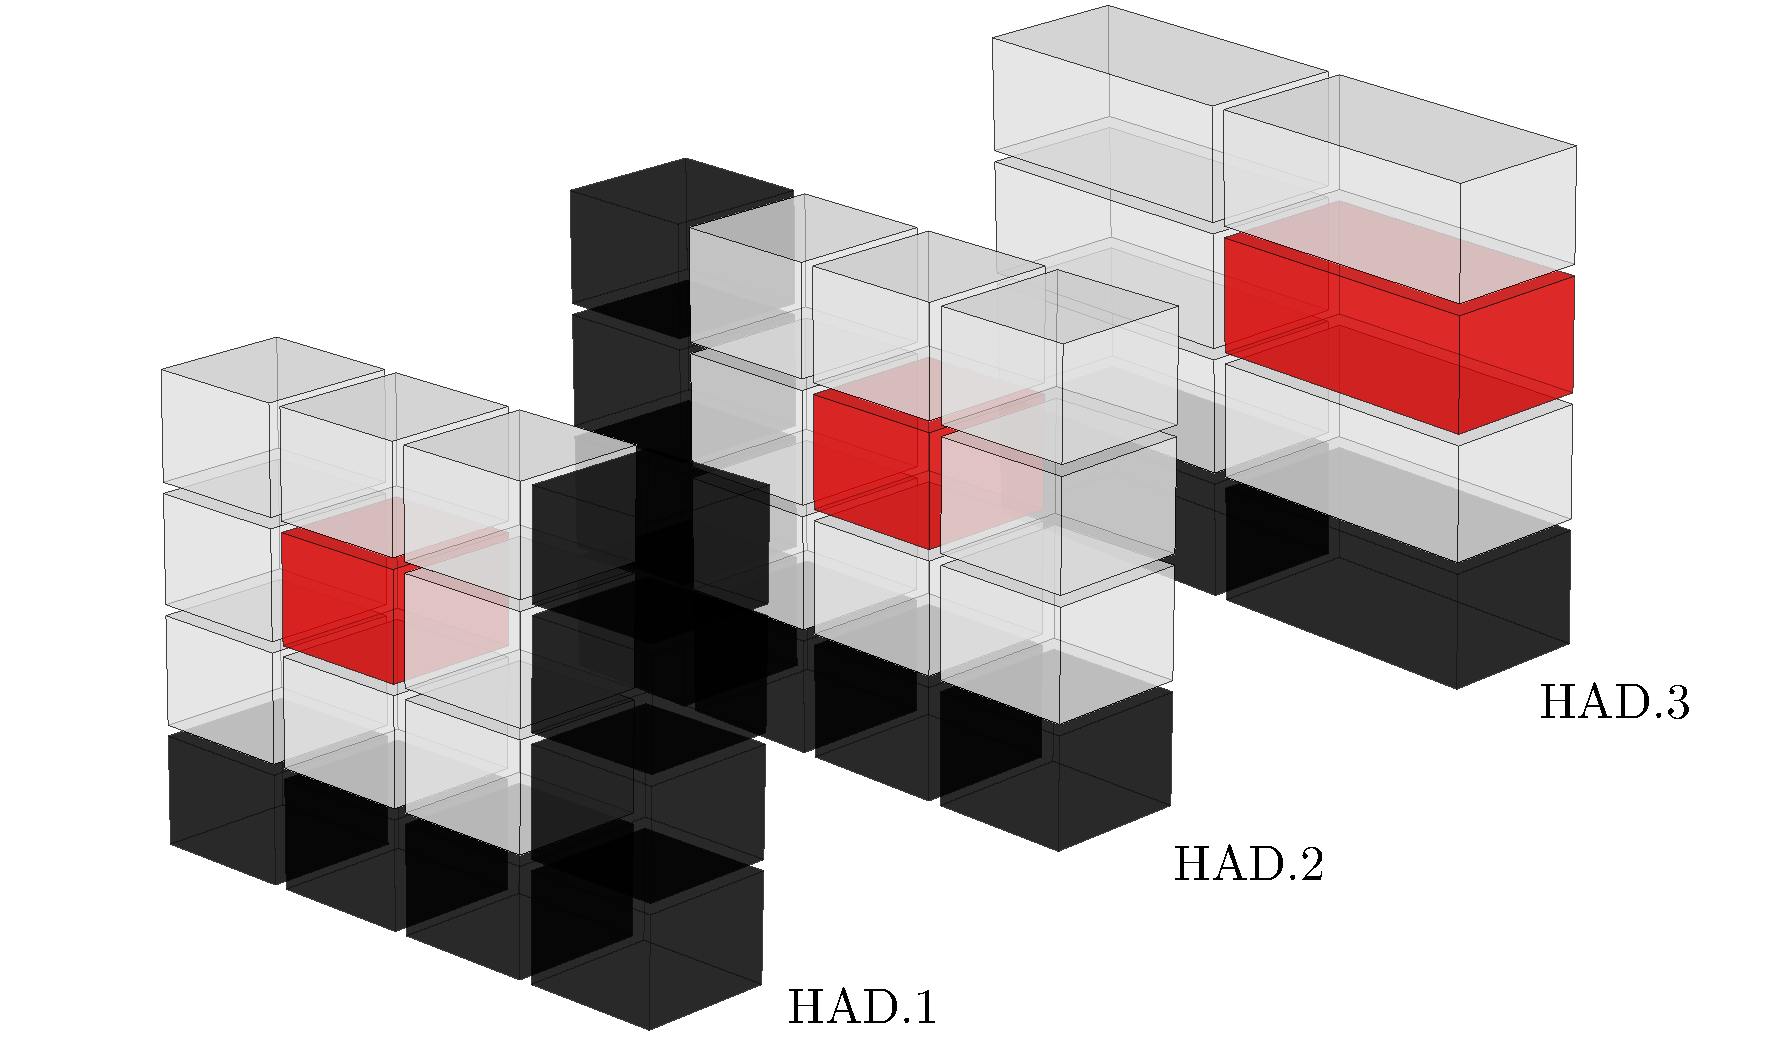
\includegraphics[width=\textwidth]{sections/ringer/figures/ATLAS_HAD_Layers_v5.pdf}
			\caption{Hadronic calorimeter cells within the ringer reconstruction window.}
		\end{subfigure}
	\end{center}
	\caption{\label{fig:calo_rings}
		Sketch to illustrate the ring-shaped energy description. See
		Section~\ref{top:algorithm} for more details. 
		The hottest cell is in red, while the consecutive neighbouring rings are represented by a cycle 
		of non-colored and black cells.
	}
\end{figure}

Nonetheless, some observations concerning the description \textcolor{red}{of a shower} through rings are
worth making. First, the standard shower shape variables (or simply shower shapes) cannot be obtained through operations starting from the rings.  Thus, the rings represent an alternative for shower development description and not a possible replacement for the shower shapes.  Therefore, a strategy considering both variables altogether (rings and shower shapes) might explore \textcolor{red}{a} complementary discriminating information in future.
%First, is not possible, by operating the rings, obtain the standard shower shapes (of simply shower shapes)}. In addition, \textcolor{red}{the rings, due to their construction, obtain similar information as the obtained from some shower shapes (i.e \rhad, \reta and \rphi).} Thus, the rings are not a replacement
%for the shower shapes and a strategy considering both variables altogether could
%explore complementary discriminating information. 
Second, one should also notice
that the rings do not use the same sensors more than once for each variable.
This is not strictly true for the shower shapes, although it is fairly unusual.
In contrast, pattern recognition through modern machine learning
algorithms~\cite{Engelbrecht2007,Goodfellow2016}, as convolution
neural-networks~\cite{Gu2018}, build variables processing several times
the same sensors. \textcolor{red}{Finally, as providing} dimension reduction and keeping the
physics interpretation of the shower development, the shower shapes \textcolor{red}{are also suited} bringing insights through univariate analysis carried out on each
single dimension composing the input space.



\section{Electron Triggers}\label{ssec:egamma_trigger}


Electron triggers~\cite{aad2020performance} begin with
the search for an EM energy deposit in the calorimeter with a \licalo{} sliding
window algorithm \textcolor{red}{~\cite{Franchino:2730851}} using coarse granularity calorimeter information, in order to
fulfill the targeted latency requirements \textcolor{red}{($2.5\mu s$)}. This selects a RoI of $0.4\times 0.4$
in the $\eta\times\phi$ axis and applies a minimal transverse energy and object
multiplicity requirements, which depend on the \textcolor{red}{trigger}
specifications~\cite{TRIG-2016-01}.
 
The \hlt{} selection starts with the fast calorimeter reconstruction
step (\fastcalo), which has two implementations
(Figure~\ref{fig:ringer_chains}): a new one based on the Ringer algorithm, which
has been operating as the baseline since 2017; and the original \textcolor{red}{cut-based
algorithm}.%~\cite{ATLAS-PERF-2017-01-002}
This processing step is followed by the fast track reconstruction
(\fastelectron), which applies restrictions on calorimeter-tracking position
matching variables. Due to its high-demanding computational \textcolor{red}{algorithms, earlier}
 fake candidates removal is specially
interesting to release CPU resources before this selection stage.


\begin{figure}[h!tb]
  \begin{center}
  %\hspace{0.01\textwidth}
  \begin{subfigure}[c]{.48\textwidth}
  \centering
  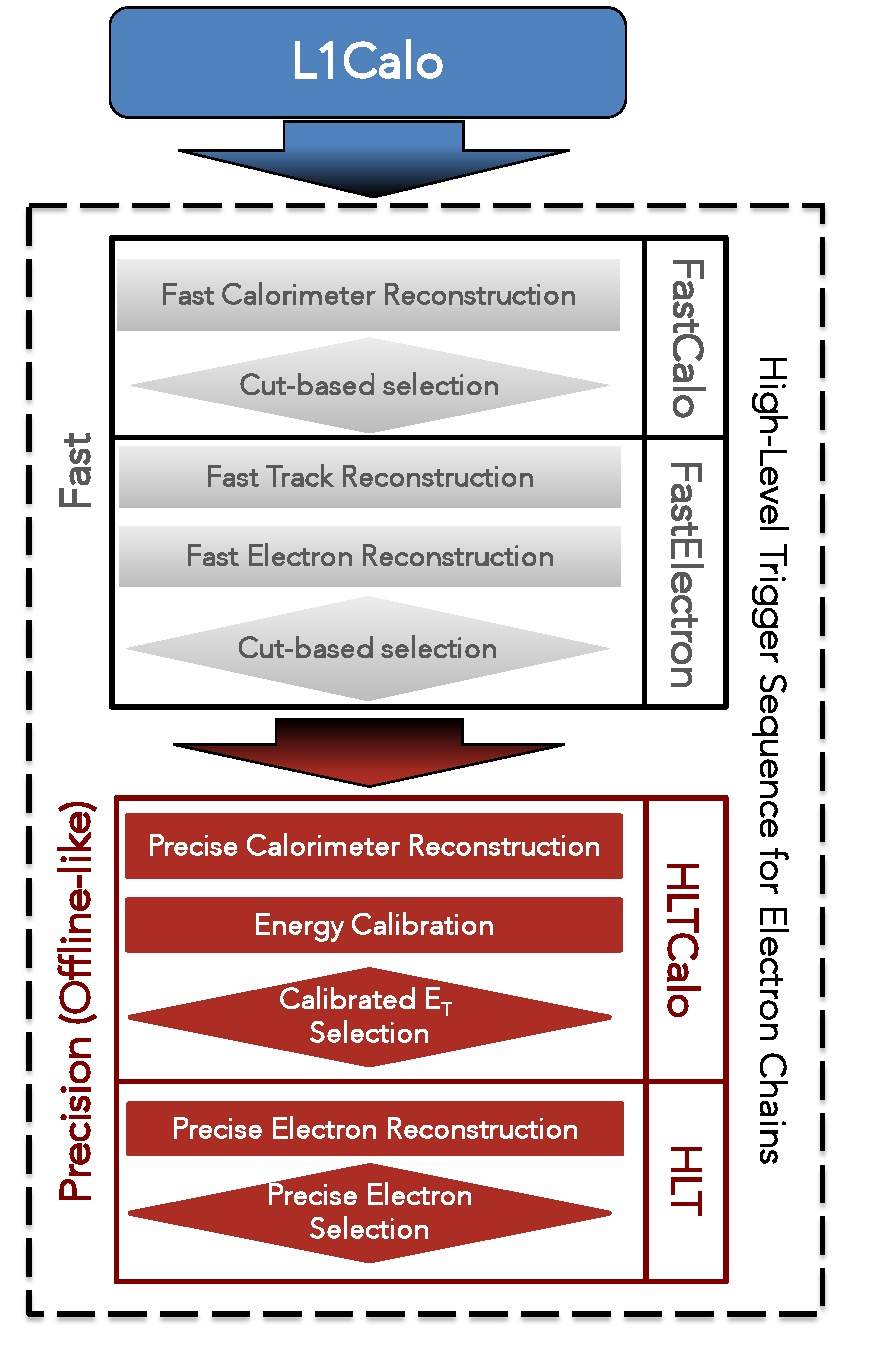
\includegraphics[width=\textwidth]{sections/context/figures/ElectronChain_Run2_cutbased.pdf}
  \caption{noringer chain (2017).}
  %\label{fig:cutbased_chain}
  \end{subfigure}
  \hfill
  \begin{subfigure}[c]{.48\textwidth}
  \centering
  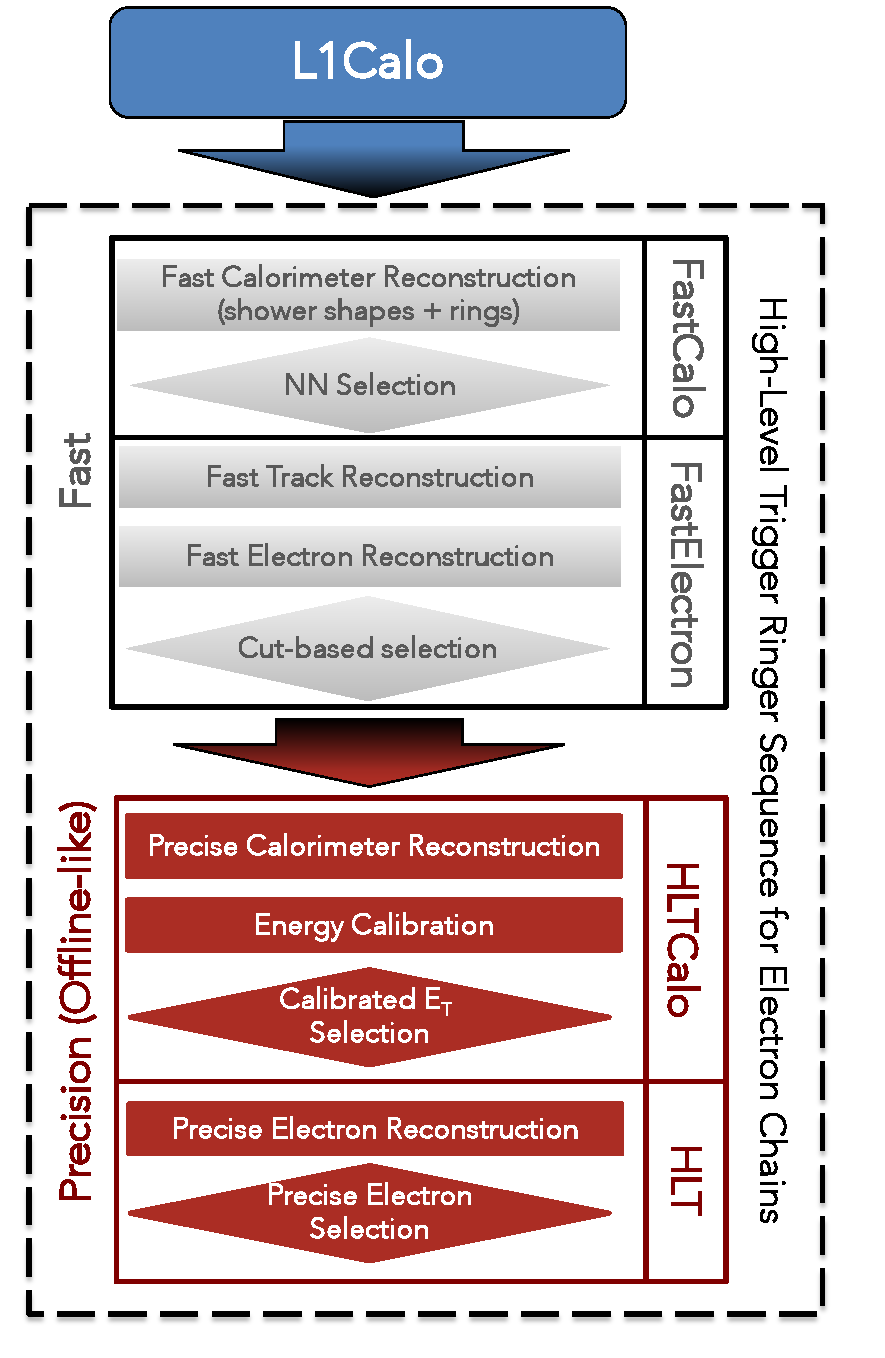
\includegraphics[width=\textwidth]{sections/context/figures/ElectronChain_Run2_ringer.pdf}
  \caption{ringer chain (2017).}
  %\label{fig:ringer_chain}
  \end{subfigure}
  %\hfill
  \caption{Comparison of the processing flow diagrams for the electron triggers. (a)
  contains the logic employed in the triggers based on the cut-based strategy
  (noringer) in the \fastcalo step. (b) contains the primary electron
  chains (ringer chains) since 2017, with the NeuralRinger algorithm.}%
  \label{fig:ringer_chains}
  \end{center}
\end{figure}

% TODO Remove column (c) or use the note table
  
  
  
This processing step is followed by the fast track reconstruction
(\fastelectron), which applies restrictions on calorimeter-tracking position
matching variables. Due to its high-demanding computational algorithms (Section~\ref{ssec:track})
, earlier fake candidates removal is specially
interesting to release CPU resources before this selection stage.

% http://acode-browser1.usatlas.bnl.gov/lxr/source/aa/Trigger/TrigHypothesis/TrigEgammaHypo/python/TrigL2CaloHypoCutDefs.py

\textcolor{red}{A precise electron candidate energy is later computed} (\hltcalo). Final HLT selection makes use of a likelihood
\textcolor{red}{approach~\cite{ATL-COM-PHYS-2017-1012,ATLAS-PERF-2017-01-002}, based} on the \textcolor{red}{estimation of marginal} probability density function \textcolor{red}{(pdf) for the discriminating variables ($\vec{x}$) given in Table~\ref{tab:IDcuts}}, which are built using adaptive Gaussian Kernel Density Estimation (KDE)~\cite{Silverman2018,TMVA}. The
resulting kernels, obtained (since 2017) from runs of the previous year, and
earlier from simulation data, are approximated by histograms with thin
granularity (generally employing 500 bins) and then interpolated to give the
signal (background) probability values computed for the $i$th \textcolor{red}{variable}
($P_{s(b),i}(x_i)$). The discriminant value is computed by

\begin{equation}
  d_{\mathcal{L}} = \frac{\mathcal{L}_{s}}{\mathcal{L}_{s} + \mathcal{L}_{b}},
\end{equation}
  
\noindent where
  
\begin{equation}
\mathcal{L}_{s(b)}(\vec{x}) = \prod_{i=1}^{n} P_{s(b),i}(x_i).
\label{eq:likelihoods}
\end{equation}

\noindent Roughly\footnote{A transformation is employed to allow
easier computation of the proper threshold~\cite{aaboud2019electron}.},
the decision is taken upon the comparison of $d_{\mathcal{L}}$ with a
threshold linearly corrected for \avgmu{}, in order to mitigate electron trigger
efficiency loss due to pile-up. In addition, some other requirements may be
applied under specific variables to improve the final
decision~\cite{aaboud2019electron}.

To account for detector response \textcolor{red}{evolution} (Section~\ref{ssec:calo}) with
respect to \Et\footnote{Projection of the energy ($E$) in the transverse plane,
computed by $E\cdot\sin(\theta)$ or $E\cdot\cosh(\eta)$.} and
$\eta$, both the KDE and discriminant requirements are computed in delimited
regions in this plane (boundaries defined in the Section~\ref{top:nn_ensemble}).
A finer-grained grid in \Et is employed for the derivation of the discriminant
requirements to obtain a relatively smooth efficiency transition. Additionally,
both pdf values and discriminant requirements near the boundaries are determined
using a linear interpolation of the neighbouring bins to avoid large
discontinuities in signal efficiency~\cite{aaboud2019electron}.

Finally, the discriminant requirements are optimized for four working points
allowing to create the operating triggers according to the desired output rate
and required efficiency: the \tight{} operating point prioritizes the purity of
collected electron candidates and demands lower output rate, while the \loose{}
and the \vloose{} ones emphasize potential electron observations, hence
resulting, specially for the latter, in higher output rate than an equivalent
tighter chain, but with substantial lower purity.  \medium{} allows a middle-term
operation between both working points. \textcolor{red}{Each} operation point also leads to
variation in the physics composition (light- and heavy-flavour, photon
conversions) of background triggered samples.




\section{Electron Trigger Nomenclature}%
\label{ssec:menu}

A set of complementary electron triggers is employed to comply with the ATLAS
physics programme~\cite{aad2020performance}. Here, we refer to the \textcolor{red}{related} nomenclature for
defining electron trigger configuration.  At HLT electron triggers are called
"$e$" followed by a value of \et-threshold used in GeV. A following set of
object identification options can be applied:



\begin{itemize}
\item $lhvloose,~lhloose,~lhmedium,~lhtight$: likelihood-based ID triggers (DEFAULT);
\item $nod0$: alignment-robust likelihood tune without \trackdO (see able~\ref{tab:IDcuts}) information (DEFAULT);
\item $etcut$: only \et-cut applied at HLT;
\item $trkcut$: require minimum number of of Si hits on track at HLT;
\item $idperf$: no track related selection.
\item $ivarloose$ is an HLT track-based isolation for electrons ($ptvarcone_{20}/p_T<0.1$).
\end{itemize}




The first two are used for physics triggers and the remaining are used
for the support triggers. Specifically, two additional options refer to
a modification in the \fastcalo{} baseline method:

\begin{itemize}
\item $ringer$: duplicated triggers using the \rnn during its
  commissioning stage in 2017 (see Section~\ref{sec:operation});
\item $noringer$: triggers employing the cut-based strategy after NeuralRinger
  commissioning stage.
\end{itemize}


Typical \licalo (e.g. EM20VHI) selection requires an EM cluster with a
given threshold (20), which can be  $\eta$-dependent within $-2$ to $+3\,$GeV
of the nominal threshold (V). Optionally, an \et-dependent veto against energy
deposited in the hadronic calorimeter behind the electron candidate's
electromagnetic cluster can be applied (H$\le \max(E_T/23-0.2, 1.0)\,$GeV), as
well as an \et-dependent electromagnetic isolation, where the effect of the
latter is compared as a function of the offline electron candidate's transverse
energy (I$\le \max(E_T/8-1.8, 2.0)\,$GeV).



\section{\TnP Method}\label{ssec:tnp}

\textcolor{red}{The \tnp{} method relies on the existence of resonances that decay to a pair of particle of interest (\Zee{}, \Jee{}, $\gamma \rightarrow ee$ and etc) ~\cite{PERF-2016-01}. In the case of electrons coming from $Z$ boson decay, the selection of two EM objects with a mass around the $Z$ mass with opposite charge is enough to get a pure sample of electrons as soon you tag one of those objects as a well identified electron. The remaining object can them be assumed to be an electron with a very high underlying purity. This object can them be used as a probe to test the electron trigger efficiency. The selection of the tag particle is done according to offline analysis criteria to make sure that the trigger selection introduces a minimal loss of those events at the final physics analysis level~\cite{aaboud2019electron}. A single electron is used to select the event at the trigger level (tag), allowing the second electron to be used as a probe to measure trigger algorithm performance~\cite{aad2020performance}.}

%One interesting problem arises when considering efficiency measurements in collision data. Without the application of a selection model, the true nature of the data is unknown and, otherwise, the measurements are biased. Fortunately, physics knowledge can shed some light to this issue. Well-known properties of physics resonances can be exploited to provide a reasonable statistical amount of electron samples for a wide kinematic range through the \tnp{} method~\cite{PERF-2016-01}. The strategy is to employ a set of requirements to ensure good quality physics objects (tag) that match the properties of a physics resonance decay when they are computed together with an additional specific physics object (probe). The resonance decays are chosen to provide probes at similar conditions expected in particular physics analysis, thus permitting to scrutinize detector behavior and eventual efficiency discrepancies between simulated and collision data. Thus, the efficiency measures computed for the Ringer were over such probes in collision data.


%One interesting problem arises when considering efficiency measurements in
%collision data. Without the application of a selection model, the true nature
%of the data is unknown and, otherwise, the measurements are biased. Fortunately,
%physics knowledge can shed some light to solve this issue. Well-known
%properties of physics resonances can be exploited to provide reasonable
%statistics amount of electron samples for a wide kinematic range through the
%\tnp{} method~\cite{PERF-2016-01}. The strategy is to employ a set of requirements
%to ensure good quality physics objects (tag) that match the properties of a
%physics resonance decay when they are computed together with an additional
%specific physics object (probe). The resonance decays are chosen to provide
%probes at similar conditions expected in particular physics analysis, thus
%permitting to scrutinize detector behavior and eventual efficiency discrepancies
%between simulated and collision data.

%\TnP{} efficiency measurements performed for the offline model selection,
%reference for physics analysis, need additional complexity to discard background 
%contamination as the method is subjected to
%inefficiency~\cite{aaboud2019electron}. The trigger system is developed to
%comply with the offline reference, culminating in higher overall system
%efficiency. Accordingly, many trigger efficiency measurements employ the \tnp
%method together with an equivalent offline requirement to increase
%their agreement and to avoid unnecessary handling of background contamination.
%This is the case of the efficiency measurements hereby reported, where the
%offline probes are matched to an equivalent trigger object and attend a specific
%offline requirment. For an unbiased evaluation of spurious signal removal and
%of the systematics involved in the electron triggers, see~\cite{aad2020performance}. 
%The \TnP{} for $Z\rightarrow$ee ressonance is described in Algorithm~\ref{alg:tap_zee},
%The offline-reconstructed electron tag must pass the following criteria:

%\begin{itemize}

%  \item It must have an associated cluster object;
%  \item It must have an associated track object;
%  \item The electron must be accepted by the offline tightness\footnote{For 2017 and 2018 we use the \textit{lhmedium} criterion. The Z mass range of the selected electron pairs was $80-100$ \GeV.} requirement;
%  \item $E_{T} > 25$ GeV;
%  \item The electron must be in the fiducial detector acceptance region;
%  \item The event must be approved by at least one of the tag triggers\footnote{Trigger tag must passed by:
%  e26\_lhtight\_nod0\_ivarloose OR e60\_lhmedium\_nod0 OR e140\_lhvloose\_nod0 OR e300\_etcut};
%  \item The tag electron must have an associated trigger object;  

%\end{itemize}

%and the offline electron probe must meet the following criteria:

%\begin{itemize}
%  \item It must have an associated cluster object;
%  \item It must have an associated track object;
%  \item It cannot have more than one jet higher than 20 GeV close\footnote{If have one jet object with $DeltaR < 0.4$ w.r.t the 
%  electron probe object, increase the counter.} to the probe electron;
%\end{itemize}

%%%%%% Coloring the comment as blue
\newcommand\mycommfont[1]{\footnotesize\ttfamily\textcolor{blue}{#1}}
\SetCommentSty{mycommfont}
\SetKwInput{KwInput}{Input}                % Set the Input
\SetKwInput{KwOutput}{Output}              % set the Output



\begin{algorithm}[H]
    \DontPrintSemicolon
    \tcc{list of all offline electrons objects in this event.}
    \KwInput{electrons} 
    \tcc{list of offline probe electrons.}
    \KwOutput{probes} 

 

    \tcc{Loop over offline tag electrons}
    \For{tag \leftarrow electrons}
    {
        \If{ it does not comply with all offline-reconstructed electron tag}
        {
            continue
        }

        \tcc{Loop over offline probe electrons}
        \For{probe \leftarrow electrons}
        {
            \If{tag = probe}
            {
                continue
            }

            \If{ tag and probe charge is the same}
            {
                continue
            }

            Mass $\leftarrow$ compute the mass of the tag and probe electron pair


            \If{ 80 GeV < Mass < 100 GeV }
            {
                \If{ it comply all offline-reconstructed electron probe }
                {
                    append probe electron into the probes list
                }

            }

        }

    }
  

\caption{Tag and Probe algorithm}
\label{alg:tap_zee}
\end{algorithm}






%Similarly, \tnp method allows to acquire collision data in order to improve
%inference, as a way to avoid limitations of the simulation in representing the
%actual experiment observations. Again, the bias arising from the offline
%requirement in the probes is expected to be beneficial to the process as a way
%of increasing the agreement of systems. On the other hand, model
%development may need to extrapolate its operation to more stringent
%pile-up conditions.

\section{Datasets and Event Selection}%
\label{ssec:dataset}

The \textcolor{red}{datasets used to train the Ringer algorithm and the event} selection \textcolor{red}{strategy used to build these signal and background samples are} available in
Table~\ref{tab:event_selection}. For a detailed description of the simulated
datasets see ~\cite[Section 3]{ATLAS-PERF-2017-01-002}. The tuning and analysis
performed on data recorded by ATLAS have their quality ensured. \textcolor{red}{The ATLAS data quality is provide through a strict Data Quality Policy that validates each part of a run dataset that can be used for analysis, rejecting any piece affected by a potential underlying inactive of dysfunctioning part of the detector.} 
In particular, periods meeting all data-quality requirements
are made available through internal files known as good run list
(GRL)~\cite{grl_site}. The physics objects were reconstructed in the first
(bulk) processing. To facilitate (big) data manipulation, events of potential
interest are derived using specific requirements. The derivation requirements
providing potential \Zee{} \tnp{} candidates, %(EGAM1), 
\Jee{} \tnp{} candidates
%(EGAM2)
 and background electrons %(EGAM7)
  were employed. The event selection was
performed by the online framework for the \textcolor{red}{\Zee{} \tnp{}} and \textcolor{red}{background electrons} derivations.%, and
%through the offline framework for the EGAM2 derivation.

% TODO Discuss how the events are selected

\begin{table}[ht!]%\footnotesize
\centering
\caption{Event selection for tuning the models and defining the discriminant
requirements of the \rnn operating in the Run 2. Symbol ``\veto'' is used to
indicate that the physics object is considered when it is rejected by the
criterion. The label `mc15' corresponds to simulated data based on Monte Carlo
algorithms and `Tier0' correspond to ATLAS experimental
data \cite{aad2020performance}.}\label{tab:event_selection}
% TODO Explain why not loose and not Zee
\resizebox{\textwidth}{!}{%
\begin{tabular}{lp{6.8cm}cc}
\hline \hline
Type & Dataset & \TnP & Offline Selection \\
\hline \hline
\multicolumn{4}{c}{2017 Models} \\
\hline
signal &
mc15\_13TeV.361106.PowhegPythia8EvtGen\allowbreak{}\_AZNLOCTEQ6L1\_Zee.merge.AOD.\allowbreak{}e3601\_s2876\_r7917\_r7676
& \Zee & None \\
background &
mc15\_13TeV.423300.Pythia8EvtGen\allowbreak{}\_A14NNPDF23LO\_perf\_JF17.merge.AOD.\allowbreak{}e3848\_s2876\_r7917\_r7676
& None & None \\
\hline
\multicolumn{4}{c}{2017 Discriminant Requirements} \\
\hline
signal & 2016 Tier0 + EGAM1 (p3013) + GRL v88 & \Zee & \tight \\
background & 2016 Tier0 + EGAM7 (p3013) + GRL v88 & \veto\Zee & \veto\loose \\
\hline
\multicolumn{4}{c}{2018 Models and Discriminant Requirements} \\
\hline
signal & 2017 Tier0 + EGAM1 (p3336) + GRL v97 & \Zee & \tight \\
background & 2017 Tier0 + EGAM7 (p3336) + GRL v97 & \veto\Zee & \veto\vloose \\
\hline \hline
\end{tabular}
}
\end{table}




